\documentclass[12pt]{paper}

\usepackage[utf8]{inputenc}
\usepackage[T1]{fontenc}
\usepackage{graphicx}
\usepackage{grffile}
\usepackage{longtable}
\usepackage{wrapfig}
\usepackage{rotating}
\usepackage[normalem]{ulem}
\usepackage{amsmath}
\usepackage{textcomp}
\usepackage{amssymb}
\usepackage{capt-of}
\usepackage{hyperref}
\usepackage{tikz}
\usepackage{bm}
\usepackage{minted}
\usepackage[margin=1in]{geometry}
\usepackage{fontspec}
\setmonofont{DejaVu Sans Mono}[Scale=MatchLowercase]

\usepackage{amsmath}
\usepackage{bm}
\usepackage{amsthm}
\usepackage{mathtools}
\usepackage{amsfonts}
\usepackage{bbm}
\usepackage{graphicx}

\DeclareMathOperator{\diam}{diam}
\DeclareMathOperator{\interior}{int}
\DeclareMathOperator{\close}{cl}

\newcommand{\met}[1]{d \left ( #1 \right )}
\newcommand{\brak}[1]{ \left [ #1 \right ] }
\newcommand{\cbrak}[1]{ \left \{ #1 \right \}}
\renewcommand{\vec}[1]{ \bm{ #1 }}
\newcommand{\abs}[1]{\left \lvert #1 \right \rvert}
\newcommand{\seq}[1]{{\left \{ #1 \right \}}}
\newcommand{\conj}[1]{ \overline{ #1 } }
%\newcommand{\close}[1]{ \bar{ #1 } }
\newcommand{\set}[1]{\left \{ #1 \right \}}
\newcommand{\Lim}{\lim\limits}
\newcommand{\compose}{\circ}
\newcommand{\inv}[1]{{#1}^{-1}}
\newcommand{\compl}[1]{{#1}^{c}}



\newcommand{\setR}{ \mathbb{R} }
\newcommand{\setQ}{ \mathbb{Q} }
\newcommand{\setZ}{ \mathbb{Z} }
\newcommand{\setN}{ \mathbb{N} }

\newcommand{\plim}{ \overset{p}{\to} }
\newcommand{\mean}[2][N]{ \overline{ #2 }_{#1}}
\newcommand{\exV}[1]{\mathbb{E} \left [ #1 \right ]}
\newcommand{\Vari}[1]{\mathbb{V} \left ( #1 \right )}

\newcommand{\est}[2][n]{ \widehat{ #2 }_{#1}}
\newcommand{\altest}[2][n]{ \tilde{ #2 }_{#1}}

\newcommand{\indicate}[1]{ \mathbbm{1}_{\{#1\}}}
\newcommand{\convDist}{ \overset{d}{\to}}
\newcommand{\unif}{\emph{U}}
\newcommand{\normal}{\mathcal{N}}
\newcommand{\eye}{\mathbbm{I}}

\newcommand{\bigO}{\mathcal{O}}
\newcommand{\Lagrange}{\mathcal{L}}

\newcommand{\deriv}[2]{\frac{ \partial #1}{ \partial #2}}

\DeclarePairedDelimiter{\ceil}{\lceil}{\rceil}
\DeclarePairedDelimiter{\floor}{\lfloor}{\rfloor}
\DeclarePairedDelimiter{\norm}{\lVert}{\rVert}

\newtheorem*{definition}{Definition}
\newtheorem{theorem}{Theorem}[section]
\newtheorem{question}{Question}
\newtheorem*{answer}{Answer}

\title{Structural Estimation Problem Set 3}
\author{Timothy Schwieg}


\newcommand\smallO{
  \mathchoice
    {{\scriptstyle\mathcal{O}}}% \displaystyle
    {{\scriptstyle\mathcal{O}}}% \textstyle
    {{\scriptscriptstyle\mathcal{O}}}% \scriptstyle
    {\scalebox{.6}{$\scriptscriptstyle\mathcal{O}$}}%\scriptscriptstyle
  }

  

\begin{document}

\maketitle

\section{Question 1}

\subsection{(a)}


To begin with, the data are loaded in.

\begin{minted}[frame=lines,fontsize=\scriptsize,xleftmargin=\parindent,linenos,mathescape,breaklines=true,stripnl=true,firstnumber=last]{julia}
incomes = DataFrame( CSV.File( "data/usincmoms.csv", delim='\t',header=[:percent,:midpoint] ) )
\end{minted}



From here, the bar chart is constructed, because of the strange shape
required in the final bins, these must be constructed manually, then
passed to the plotting library as a bar chart.



\begin{minted}[frame=lines,fontsize=\scriptsize,xleftmargin=\parindent,linenos,mathescape,breaklines=true,stripnl=true,firstnumber=last]{julia}
heights = copy(incomes[:percent])
heights[41] /= 10.0
heights[42] /= 20.0

bins = Vector{Int64}(undef,length(incomes[:midpoint])+1)
bins[1] = 0
for i in 1:length(incomes[:midpoint])
    bins[i+1] = bins[i] + ((incomes[:midpoint][i]) - bins[i])*2
end

plotBins = copy(bins)
plotBins ./= 1000.0

plot( plotBins, heights, bins = bins, seriestype=:barbins, xlabel="Thousands of Dollars", label="US Incomes", ylabel="density")

savefig("histogram.pdf")
\end{minted}

% Insert the picture here
\begin{centering}
  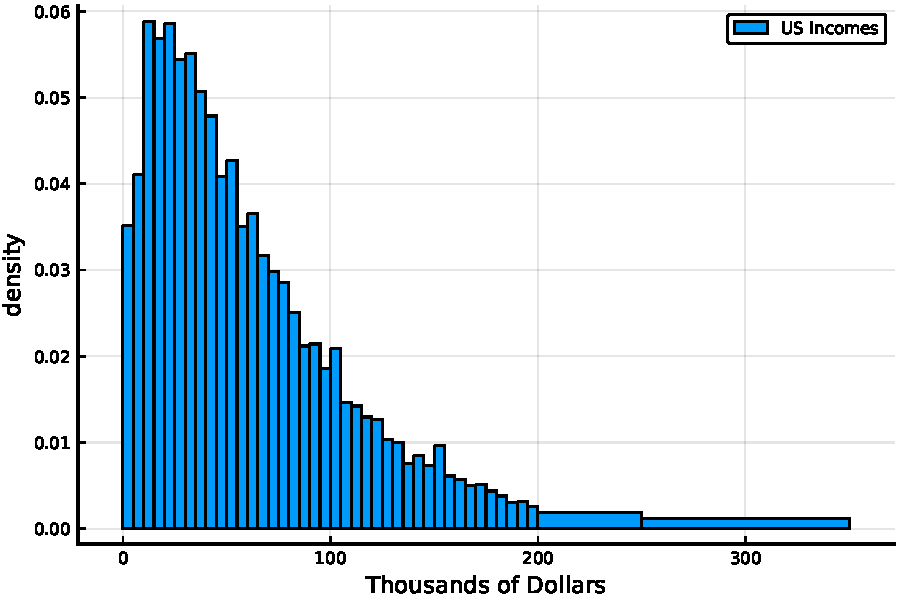
\includegraphics{histogram.pdf}
\end{centering}

We can see that there is a tail to this distribution, though not
nearly as long as in the health distribution.

\subsection{(b)}

We wish to fit the log-normal distribution to the data, using the mass
in each of the bins as the moment criterion. As such, this
optimization can be understood as the question of:

\begin{align*}
  \min_{\mu,\sigma} \quad &e' W e\\
  \text{ s.t. } \quad & e_i = \int_{b_{i-1}}^{b_i} dF(\mu,\sigma) - m_i
\end{align*}

Where $W$ is a given weighting matrix, $b_i$ are the cut-off points
for the bins, $b_0 = 0$, and $m_i$ are the moments recorded in the
data. This is implemented below in full distribution generality, and
then applied for the specific Log-Normal Distribution.

\begin{minted}[frame=lines,fontsize=\scriptsize,xleftmargin=\parindent,linenos,mathescape,breaklines=true,stripnl=true,firstnumber=last]{julia}
container = Vector{Float64}(undef,42)


function GenerateMoments( container::Vector{Float64},bins::Vector{Float64},
                                   distribution, params::Vector)
    cdfs = [cdf( distribution(params...), x) for x in bins]

    for i in 1:42
        container[i] = cdfs[i+1] - cdfs[i]
    end
    return container
end

W = convert( Matrix{Float64}, Diagonal(convert(Vector{Float64}, incomes[:percent])) )

function GMMCrit( W::Matrix{Float64}, dataMoments::Vector{Float64},
                  container::Vector{Float64}, bins::Vector{Float64},
                  distributions, params::Vector)
    e = GenerateMoments( container, bins, distributions, params ) - dataMoments
    return dot(e, W*e)#e'*W*e
end
\end{minted}

The question remains as to what should be used as a starting point for
our optimization algorithm. To this end, I simulate from the
multinomial distribution defined by the bins, and calculate the
Method-of-Moments estimators for the log-normal distribution from this
simulated data. These estimators take the form of:
\begin{align*}
  \est{\sigma}^2 &= \log \frac{s^2}{\mean{x} + 1}\\
  \est{\mu} &= \log \mean{x} - \frac{\est{\sigma}^2}{2}
\end{align*}

This is implemented below:
\begin{minted}[frame=lines,fontsize=\scriptsize,xleftmargin=\parindent,linenos,mathescape,breaklines=true,stripnl=true,firstnumber=last]{julia}
dataProbs = cumsum( incomes[:percent])
dataProbs[length(dataProbs)] = 1.0
N = 100000
M = length(dataProbs)
simulation = rand( Uniform(), N)
for i in 1:N
    for j in 1:M
        if( simulation[i] < dataProbs[j])
            simulation[i] = incomes[:midpoint][j]
            break
        end
    end
end

simMean = mean(simulation)
simVar = var(simulation)

sigGuess = log( simVar / (simMean*simMean) + 1)
muGuess = log(simMean) - sigGuess / 2.0
\end{minted}

Using these points as the starting points for our optimization
algorithm, we can then compute the minimizers for the GMM criterion
function.

\begin{minted}[frame=lines,fontsize=\scriptsize,xleftmargin=\parindent,linenos,mathescape,breaklines=true,stripnl=true,firstnumber=last]{julia}
dataStuff = convert(Vector{Float64}, incomes[:percent])
cdfBins = convert(Vector{Float64}, bins)

θ = [muGuess, sqrt(sigGuess)]
fun(x::Vector) = GMMCrit( W, dataStuff, container, cdfBins, LogNormal, x  )

logResult = optimize( fun, θ, BFGS())
\end{minted}

The results from the optimization are printed below:

\begin{verbatim}
Results of Optimization Algorithm
 * Algorithm: BFGS
 * Starting Point: [10.818767925970231,0.7701372401373785]
 * Minimizer: [10.862298881282367,1.022995942443407]
 * Minimum: 3.522920e-05
 * Iterations: 7
 * Convergence: true
   * |x - x'| ≤ 0.0e+00: false 
     |x - x'| = 1.54e-05 
   * |f(x) - f(x')| ≤ 0.0e+00 |f(x)|: false
     |f(x) - f(x')| = 1.07e-08 |f(x)|
   * |g(x)| ≤ 1.0e-08: true 
     |g(x)| = 3.07e-11 
   * Stopped by an increasing objective: false
   * Reached Maximum Number of Iterations: false
 * Objective Calls: 27
 * Gradient Calls: 27
\end{verbatim}

We now overlay the histogram of $\mu,\sigma$ on the bar chart used to display
the data from part (a).
\begin{minted}[frame=lines,fontsize=\scriptsize,xleftmargin=\parindent,linenos,mathescape,breaklines=true,stripnl=true,firstnumber=last]{julia}
mu = logResult.minimizer[1]
sigma = logResult.minimizer[2]

estHeightsLoggyBoy = GenerateMoments( container, cdfBins, LogNormal, [mu, sigma] )
estHeightsLoggyBoy[41] /= 10.0
estHeightsLoggyBoy[42] /= 20.0

plot!(incomes[:midpoint], estHeightsLoggyBoy, label="LogNormal GMM Estimate")
\end{minted}

\begin{centering}
  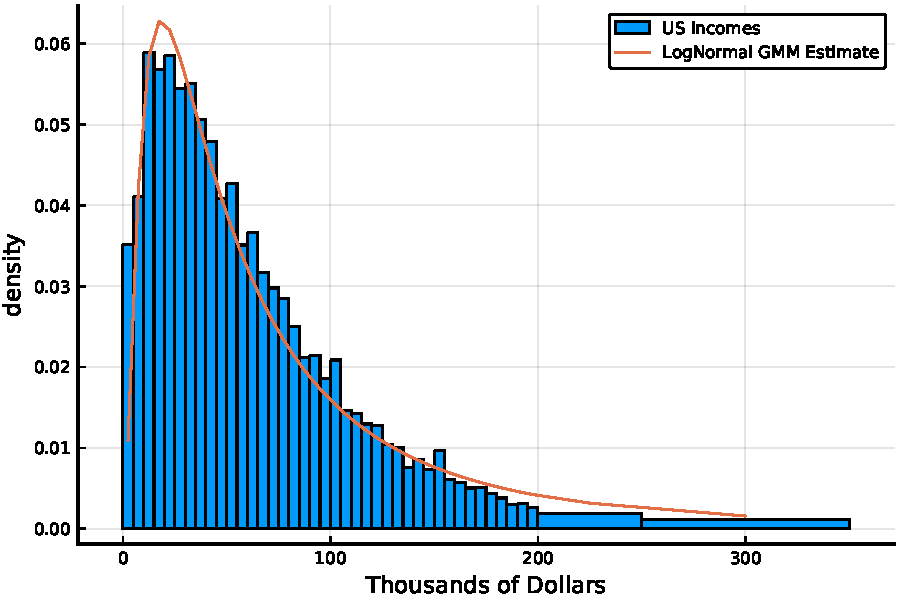
\includegraphics{loggyboy.pdf}
\end{centering}

\subsection{(c)}

For the Gamma Distribution, we are given initial values to choose, and
can implement our estimation using the same function as before, with
simply changing the distribution that is passed.

\begin{minted}[frame=lines,fontsize=\scriptsize,xleftmargin=\parindent,linenos,mathescape,breaklines=true,stripnl=true,firstnumber=last]{julia}
gamContainer = copy(container)
θ = [3.0, 25000.0]
betaFun(x::Vector) = GMMCrit( W, dataStuff, gamContainer, cdfBins, Gamma, x  )
gamResult = optimize( betaFun, θ, BFGS())
\end{minted}

The results for our optimization algorithm are printed below:

\begin{verbatim}
Results of Optimization Algorithm
 * Algorithm: BFGS
 * Starting Point: [3.0,25000.0]
 * Minimizer: [1.3984481398133792,46486.004874968334]
 * Minimum: 1.094699e-05
 * Iterations: 13
 * Convergence: true
   * |x - x'| ≤ 0.0e+00: false 
     |x - x'| = 6.37e+00 
   * |f(x) - f(x')| ≤ 0.0e+00 |f(x)|: false
     |f(x) - f(x')| = 7.44e-06 |f(x)|
   * |g(x)| ≤ 1.0e-08: true 
     |g(x)| = 1.91e-09 
   * Stopped by an increasing objective: false
   * Reached Maximum Number of Iterations: false
 * Objective Calls: 52
 * Gradient Calls: 52
\end{verbatim}

The histogram is plotted in the same way as before as well:

\begin{minted}[frame=lines,fontsize=\scriptsize,xleftmargin=\parindent,linenos,mathescape,breaklines=true,stripnl=true,firstnumber=last]{julia}
estHeightsGammaMan = GenerateMoments( gamContainer, cdfBins, Gamma, [gamAlpha, gamBeta] )
estHeightsGammaMan[41] /= 10.0
estHeightsGammaMan[42] /= 20.0

plot!(incomes[:midpoint] / 1000.0, estHeightsGammaMan, label="Gamma GMM Estimate")
\end{minted}

\begin{centering}
  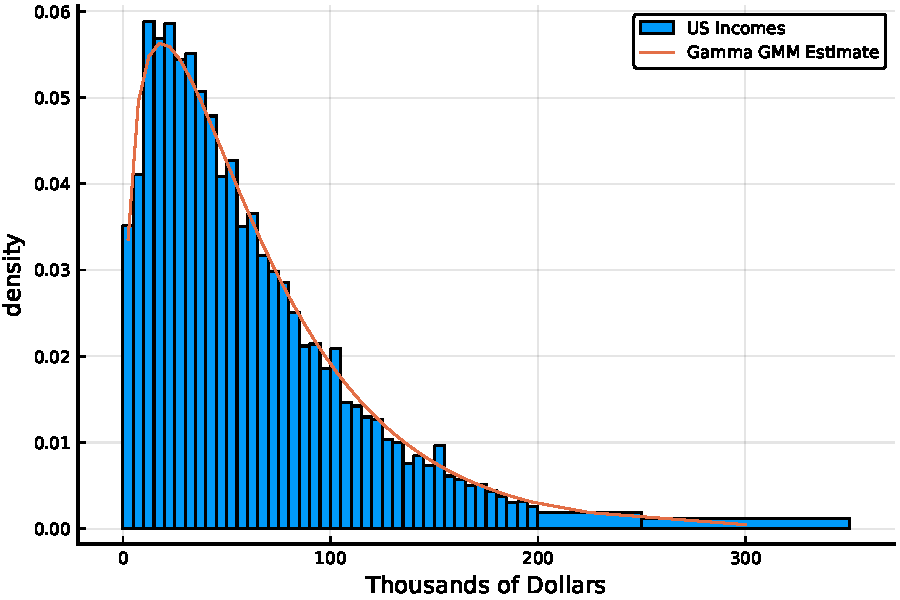
\includegraphics{gammaMan.pdf}
\end{centering}

\subsection{(d)}

The overlaid plots are shown below:

% I WANT PHOTOS OF SPIDER MAN NOW
\begin{centering}
  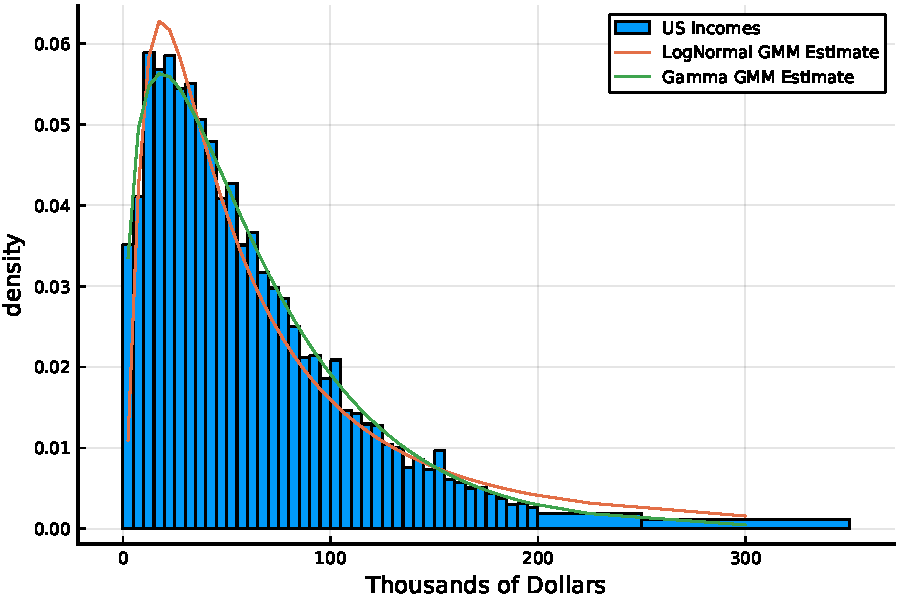
\includegraphics{allTogetherNow.pdf}
\end{centering}


The question of the most precise way to tell which distribution fits
the data the best is subjective. To define ``best'' we need to define
a norm. The norm that these moments are minimized on is the sample
frequency, and based upon this norm, which distribution fits the data
best is simply which has a smaller minimum. By this norm we find that
the Gamma Distribution is the better fit.

\vspace{.25in}
\begin{tabular}{ll}
  Gamma Minimum & $1.09470 \times 10^{-5}$\\
  LogNormal Minimum & $3.52292 \times 10^{-5}$\\
\end{tabular}
\vspace{.25in}

However, this is not a common norm used when describing the distance
between two distributions. More common notions of distance are the
total-variation norm, or the kullback-leibler
distance. However since the latter is not an actual norm, we will
consider the total variation norm, which is commonly used to compute
the ``distance'' between two distributions.

\begin{minted}[frame=lines,fontsize=\scriptsize,xleftmargin=\parindent,linenos,mathescape,breaklines=true,stripnl=true,firstnumber=last]{julia}
sum(abs(x - y) for (x,y) in zip( estHeightsGammaMan, dataStuff)) / 2

sum(abs(x - y) for (x,y) in zip( estHeightsLoggyBoy, dataStuff)) / 2
\end{minted}



\begin{tabular}{ll}
  Gamma Norm & $0.048159$\\
  LogNormal Norm & $0.071237$
\end{tabular}

\vspace{.25in}

Under this norm, we find that the Gamma fits the data better as
well. These are both in line with the visual test, which appears to
show the gamma distribution fitting the data better.

\section{Question 2}

The empirical analogs to our estimates are obtained by the
analogy-principle. From the WLLN we know that we can replace
expectations with averages, and the results will converge in
probability. Following this logic our moment conditions that we are
minimizing with respect to are:

\begin{align*}
  \frac{1}{T} \sum_{t=1}^T \brak{ z_{t+1} - \rho z_t - (1-\rho)\mu} &= 0\\
  \frac{1}{T} \sum_{t=1}^T \brak{ \left( z_{t+1} - \rho z_t - (1-\rho)\mu
  \right)z_t} &= 0\\
  \frac{1}{T} \sum_{t=1}^T \brak{ \beta \alpha \exp(z_{t+1}) k_{t+1}^{\alpha-1}
  \frac{c_t}{c_{t+1}} - 1} &= 0\\
  \frac{1}{T} \sum_{t=1}^T \brak{ \left( \beta \alpha \exp(z_{t+1}) k_{t+1}^{\alpha-1}
  \frac{c_t}{c_{t+1}} - 1 \right) w_t} &= 0\\  
\end{align*}

For our initial guess, we will use the estimates that we reached
during Problem Set 2.

\begin{minted}[frame=lines,fontsize=\scriptsize,xleftmargin=\parindent,linenos,mathescape,breaklines=true,stripnl=true,firstnumber=last]{julia}
macroData = DataFrame(load("data/MacroSeries.csv", header_exists=false, colnames=["C", "K", "W", "R"]))

function ConstructMoments( moments::Vector{Real}, α::Real, β::Real, ρ::Real,
                           μ::Real, c::Vector{Float64},k::Vector{Float64},
                           w::Vector{Float64}, r::Vector{Float64}, W::Matrix{Real})
    # $r_t - \alpha \exp ( z_t ) k_t^{\alpha - 1} = 0$
    # $\log r_t = \log \alpha + z_t + (\alpha - 1) \log k_t$
    # $z_t = \log r_t - \log \alpha - (\alpha - 1) \log k_t$
    N = 100
    z = Vector{Real}(undef, N)
    for i in 1:N
        z[i] = log( r[i]) - log(α) - (α - 1.0)*log( k[i] )
    end

    moments[1] = mean( z[i+1]- ρ*z[i] - (1-ρ)*μ for i in 1:99)
    moments[2] = mean( (z[i+1]- ρ*z[i] - (1-ρ)*μ)*z[i] for i in 1:99)
    moments[3] = mean( β * α * exp(z[i+1]) * k[i+1]^(α-1.0) * (c[i]/c[i+1]) - 1 for i in 1:99)
    moments[4] = mean( (β*α*exp(z[i+1])*k[i+1]^(α-1.0) * (c[i]/c[i+1]) - 1)*w[i] for i in 1:99 )

    return sum(moments[i]*moments[i] for i in 1:4)
end

function limitedLogistic( unbounded::Real )
    return ((exp(unbounded)) / ( 1 + exp(unbounded)))*.99 + .005
end

function invertLogistic( x::Real )
    return log( (1.0-200.0*x)/ (200.0*x - 199.0))
end

W = convert(Matrix{Real}, Diagonal([1.0,1.0,1.0,1.0]))

c = convert( Vector{Float64}, macroData[:C] )
w = convert( Vector{Float64}, macroData[:W] )
k = convert( Vector{Float64}, macroData[:K] )
r = convert( Vector{Float64}, macroData[:R] )

mom = Vector{Real}(undef,4)

#Initialize this guy with the stuff we got the first time around
alphaStart = invertLogistic(.70216)
rhoStart = atanh(.47972)
muStart = log(5.0729)

θ = [alphaStart, rhoStart, muStart]

f(x::Vector) = ConstructMoments( mom, limitedLogistic(x[1]), tanh(x[2]), exp(x[3]), .99, c, k, w, r, W )

result = optimize( f, θ, Newton(), autodiff = :forward)

alphaHat = limitedLogistic( result.minimizer[1])
rhoHat = tanh( result.minimizer[2])
muHat = exp( result.minimizer[3])
\end{minted}

Output from the optimization algorithm is given below:

\begin{verbatim}
Results of Optimization Algorithm
 * Algorithm: Newton's Method
 * Starting Point: [0.8673885548750386,0.5226205157374497, ...]
 * Minimizer: [0.8713799716017797,0.5214436286856307, ...]
 * Minimum: 3.467430e-19
 * Iterations: 9
 * Convergence: true
   * |x - x'| ≤ 0.0e+00: false 
     |x - x'| = 1.05e-05 
   * |f(x) - f(x')| ≤ 0.0e+00 |f(x)|: false
     |f(x) - f(x')| = 7.09e+03 |f(x)|
   * |g(x)| ≤ 1.0e-08: true 
     |g(x)| = 1.33e-11 
   * Stopped by an increasing objective: false
   * Reached Maximum Number of Iterations: false
 * Objective Calls: 27
 * Gradient Calls: 27
 * Hessian Calls: 9
\end{verbatim}

However these minimizers are points in $\setR^3$, so they must be
translated back into the parameter space. The output from this is
given below.

\begin{center}
  \begin{tabular}{rr}
    Criterion: & $3.467 \times 10^{-19}$\\
\(\est{\alpha}\): & 0.70298\\
\(\est{\rho}\): & 0.47881\\
\(\est{\mu}\): & 5.05981\\
\end{tabular}
\end{center}


\end{document}
